\documentclass[12pt,a4paper]{article}
\usepackage[polish]{babel}
\usepackage[T1]{fontenc}
\usepackage{lmodern}
\usepackage[utf8x]{inputenc}
\usepackage{hyperref}
\usepackage{url}
\usepackage{graphicx}
\usepackage{listings}
\usepackage{xcolor}

\colorlet{punct}{red!60!black}
\definecolor{background}{HTML}{EEEEEE}
\definecolor{delim}{RGB}{20,105,176}
\definecolor{bluekeywords}{rgb}{0,0,1}
\definecolor{greencomments}{rgb}{0,0.5,0}
\definecolor{redstrings}{rgb}{0.64,0.08,0.08}
\definecolor{xmlcomments}{rgb}{0.5,0.5,0.5}
\definecolor{types}{rgb}{0.17,0.57,0.68}
\colorlet{numb}{magenta!60!black}
\lstdefinelanguage{Kotlin}{
  comment=[l]{//},
  commentstyle={\color{gray}\ttfamily},
  emph={delegate, filter, first, firstOrNull, forEach, lazy, map, mapNotNull, println, return@},
  emphstyle={\color{OrangeRed}},
  identifierstyle=\color{black},
  keywords={abstract, actual, as, as?, break, by, class, companion, continue, data, do, dynamic, else, enum, expect, false, final, for, fun, get, if, import, in, interface, internal, is, null, object, override, package, private, public, return, set, super, suspend, this, throw, true, try, typealias, val, var, vararg, when, where, while},
  keywordstyle={\color{NavyBlue}\bfseries},
  morecomment=[s]{/*}{*/},
  morestring=[b]",
  morestring=[s]{"""*}{*"""},
  ndkeywords={@Deprecated, @JvmField, @JvmName, @JvmOverloads, @JvmStatic, @JvmSynthetic, Array, Byte, Double, Float, Int, Integer, Iterable, Long, Runnable, Short, String},
  ndkeywordstyle={\color{BurntOrange}\bfseries},
  sensitive=true,
  stringstyle={\color{ForestGreen}\ttfamily},
}
\lstdefinelanguage{json}{
    basicstyle=\normalfont\ttfamily,
    numbers=left,
    numberstyle=\scriptsize,
    stepnumber=1,
    numbersep=8pt,
    showstringspaces=false,
    breaklines=true,
    frame=lines,
    backgroundcolor=\color{background},
    literate=
     *{0}{{{\color{numb}0}}}{1}
      {1}{{{\color{numb}1}}}{1}
      {2}{{{\color{numb}2}}}{1}
      {3}{{{\color{numb}3}}}{1}
      {4}{{{\color{numb}4}}}{1}
      {5}{{{\color{numb}5}}}{1}
      {6}{{{\color{numb}6}}}{1}
      {7}{{{\color{numb}7}}}{1}
      {8}{{{\color{numb}8}}}{1}
      {9}{{{\color{numb}9}}}{1}
      {:}{{{\color{punct}{:}}}}{1}
      {,}{{{\color{punct}{,}}}}{1}
      {\{}{{{\color{delim}{\{}}}}{1}
      {\}}{{{\color{delim}{\}}}}}{1}
      {[}{{{\color{delim}{[}}}}{1}
      {]}{{{\color{delim}{]}}}}{1},
}

\title{Game Of Life\\Aplikacje Mobilne - Projekt Zespołowy}
\author{Artur Bednarczyk, Dawid Grajewski, Tomasz Januszek\\Politechnika Śląska\\Wydział Matematyki Stosowanej\\Informatyka, semestr VI}
\date{\today}

\begin{document}
\maketitle
\newpage
\tableofcontents
\newpage
\section{O projekcie}
\subsection{Zespół}
\begin{tabular}{c|l}
Osoba & Główna odpowiedzialność \\
\hline
Artur Bednarczyk & Organizacja, dokumentacja, film \\
Dawid Grajewski &  \\
Tomasz Januszek & 
\end{tabular}
\subsection{Temat}
\paragraph{Gra w życie Conwaya}
Wizualizacja ciągła i krokowa (zmienna szybkość), możliwość odczytu i zapisu planszy, różne rozmiary planszy, dostosowywanie planszy do różnych ekranów urządzeń mobilnych.
	
	Bonus: konfigurowalne reguły gry z uwzględnieniem wersji kolorystycznych.

\section{Projekt}
\subsection{UI/UX}
\subsubsection{Zawartość}
UI programu będzie złożone z kilku elementów:
\begin{itemize}
	\item Splash Screen - ekran powitalny
	\item Menu - pozwoli na przejście do konkretnych opcji aplikacji.
	\item Ustawienia - w tym miejscu użytkownik może zmienić reguły gry, kolorystykę oraz rozmiar planszy.
	\item O Projekcie - Informacje o projekcie oraz krótka instrukcja.
	\item Wczytywanie - Lista zapisanych stanów gry.
	\item Gra - Widok planszy oraz ustawień prędkości. Tutaj również użytkownik może zapisać stan gry.
\end{itemize}
\subsubsection{Projekty UI}
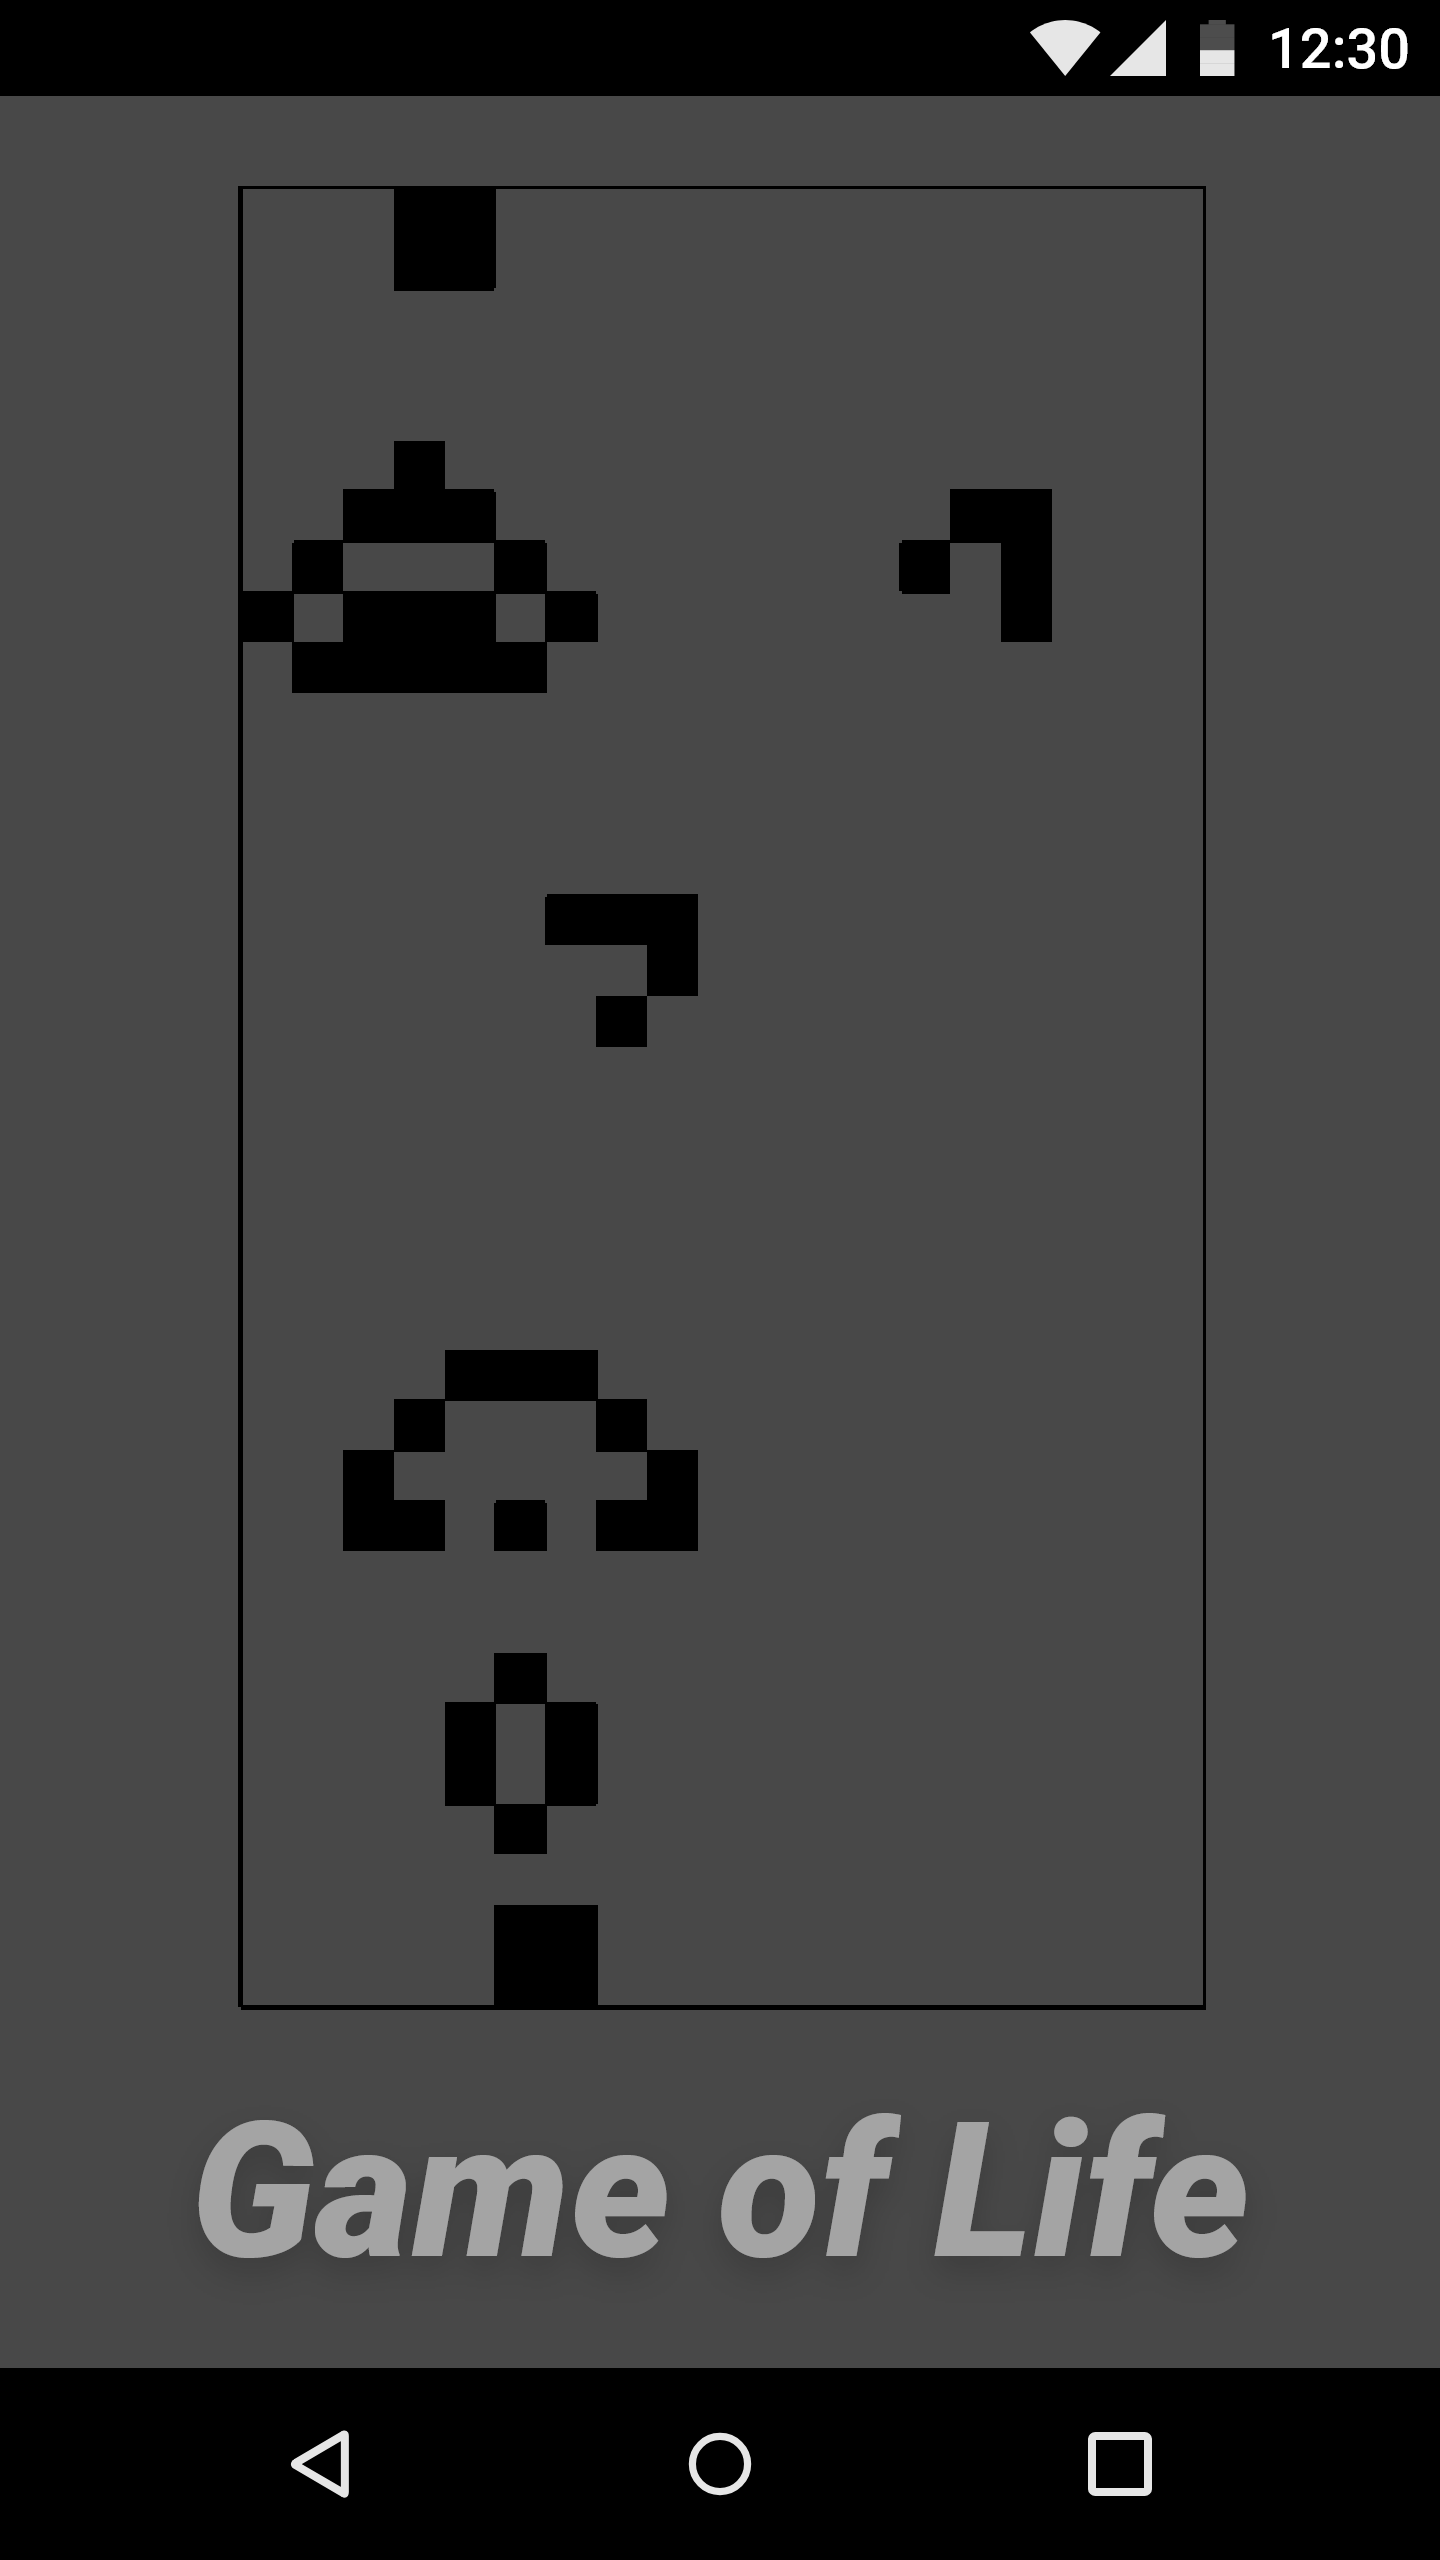
\includegraphics[width=0.33\textwidth]{Images/ui_splash.png}
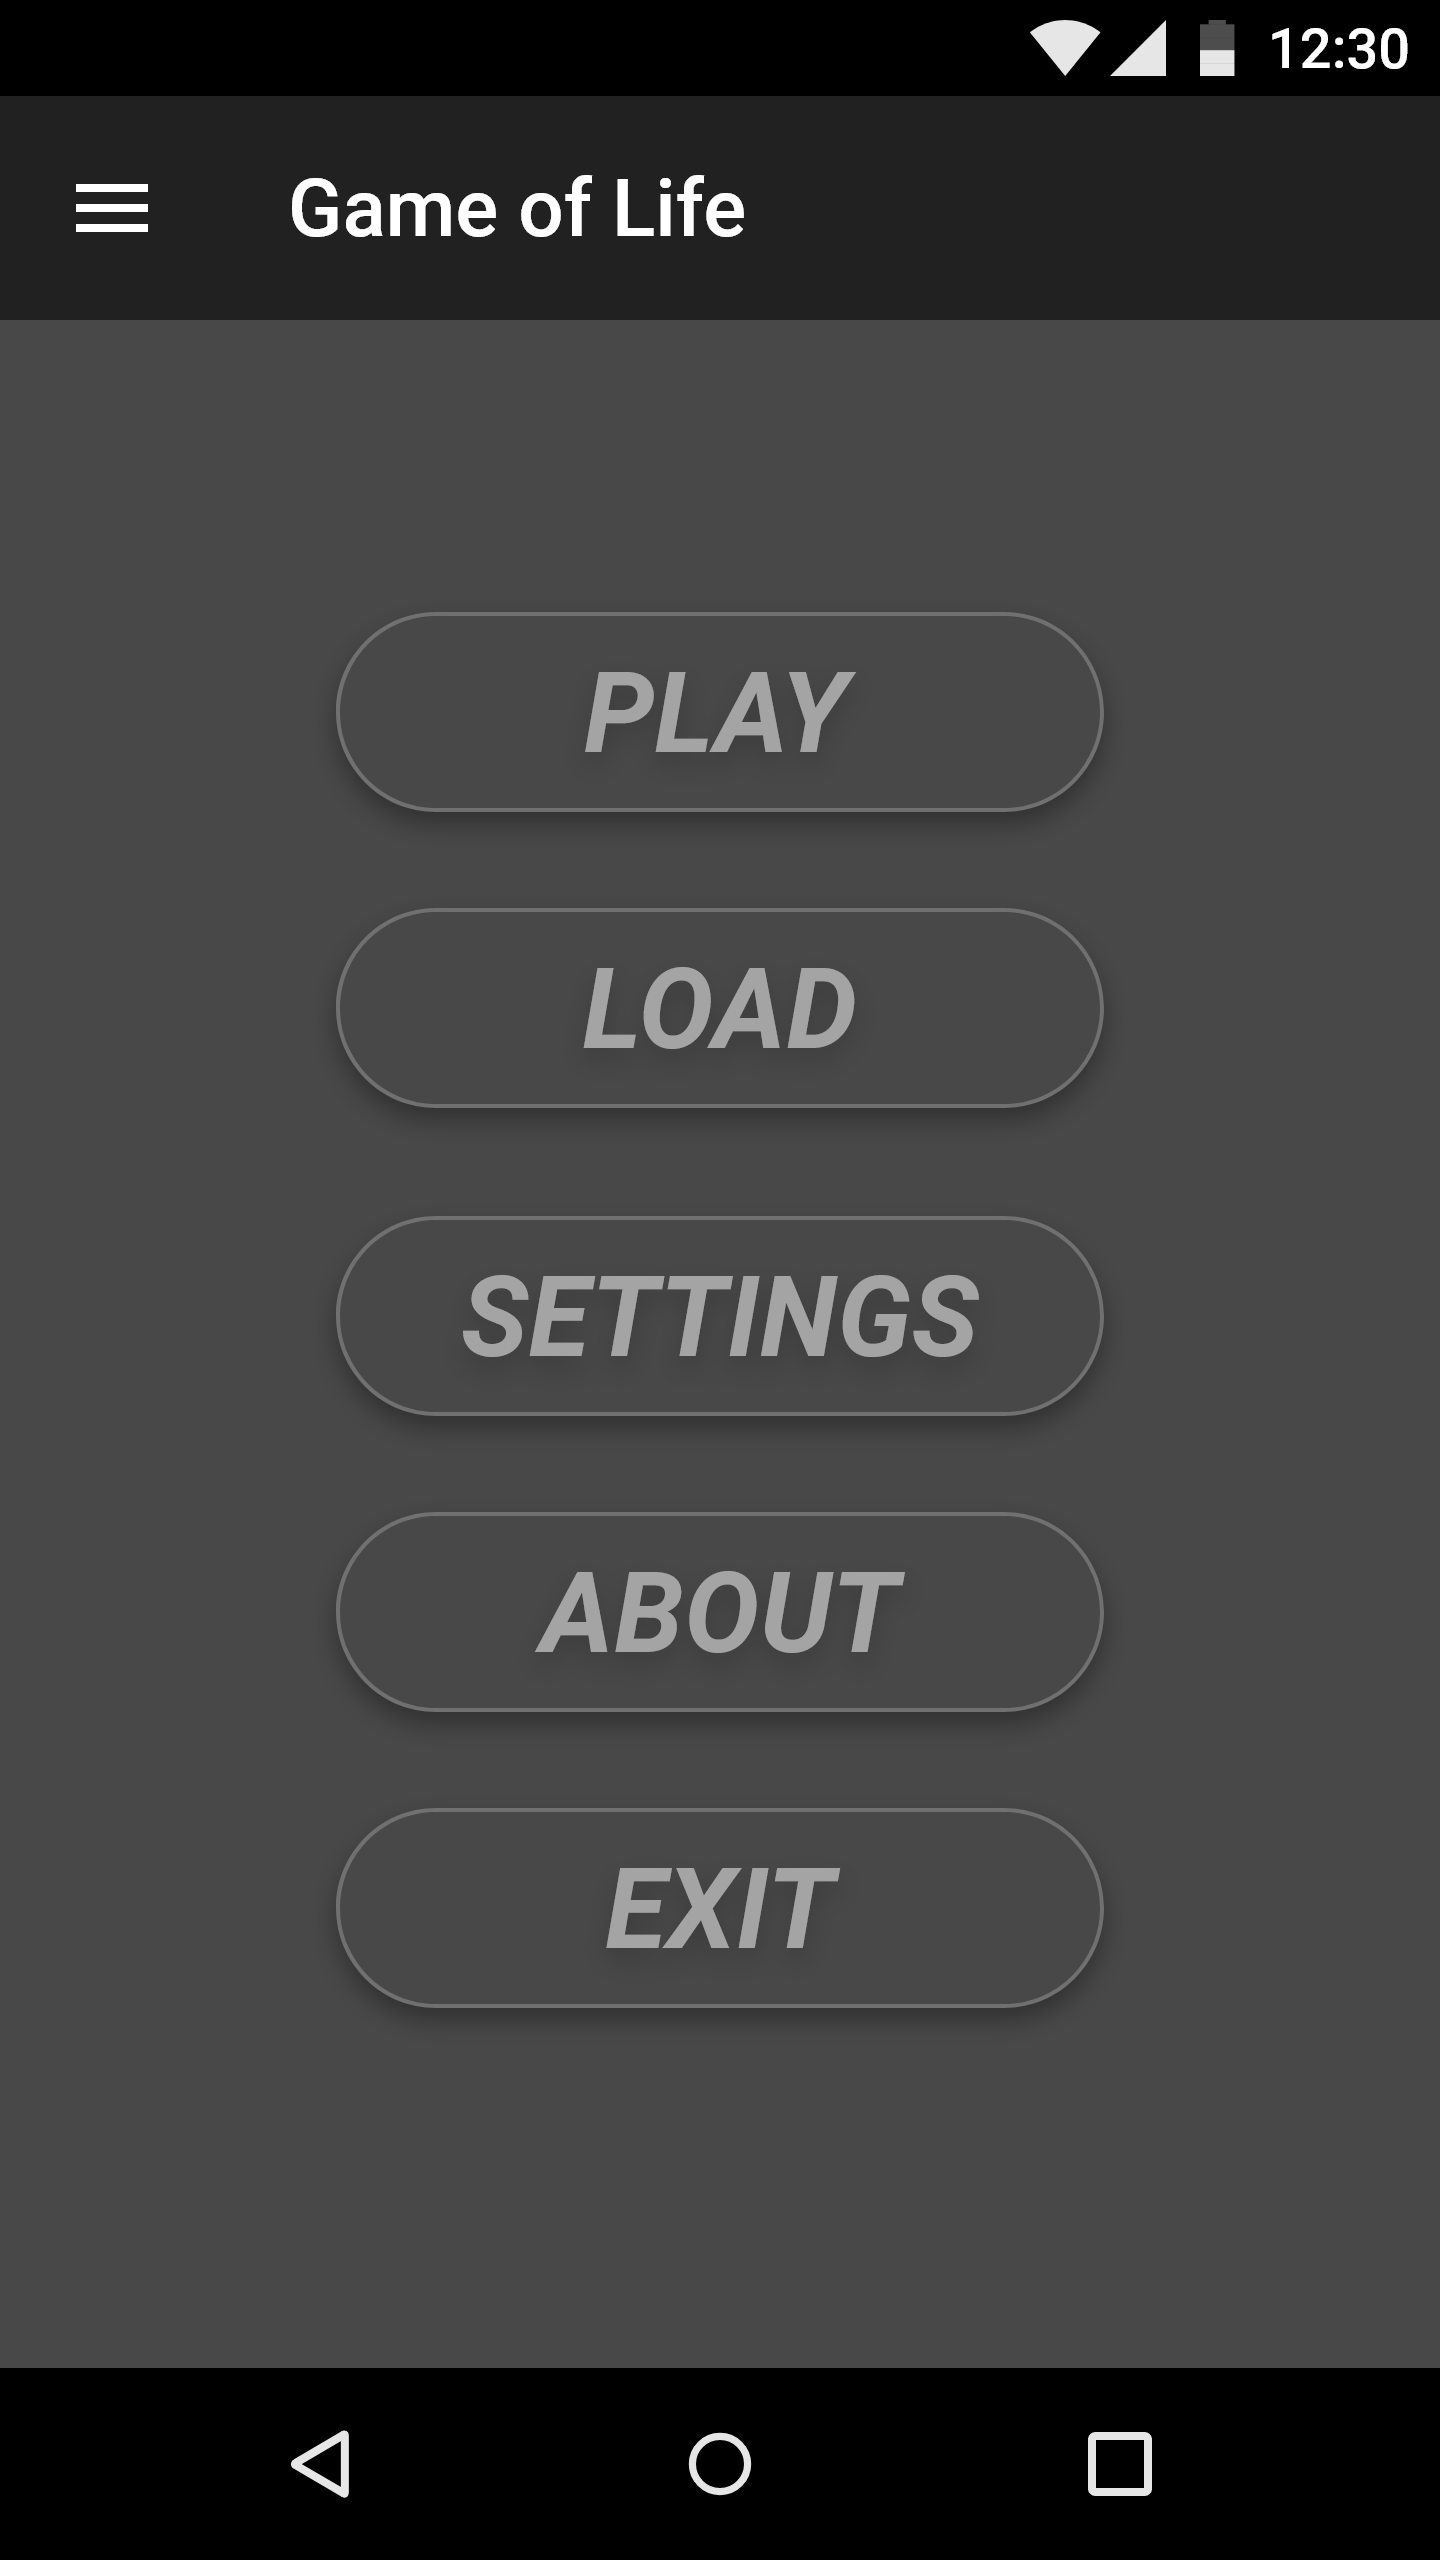
\includegraphics[width=0.33\textwidth]{Images/ui_main.png}
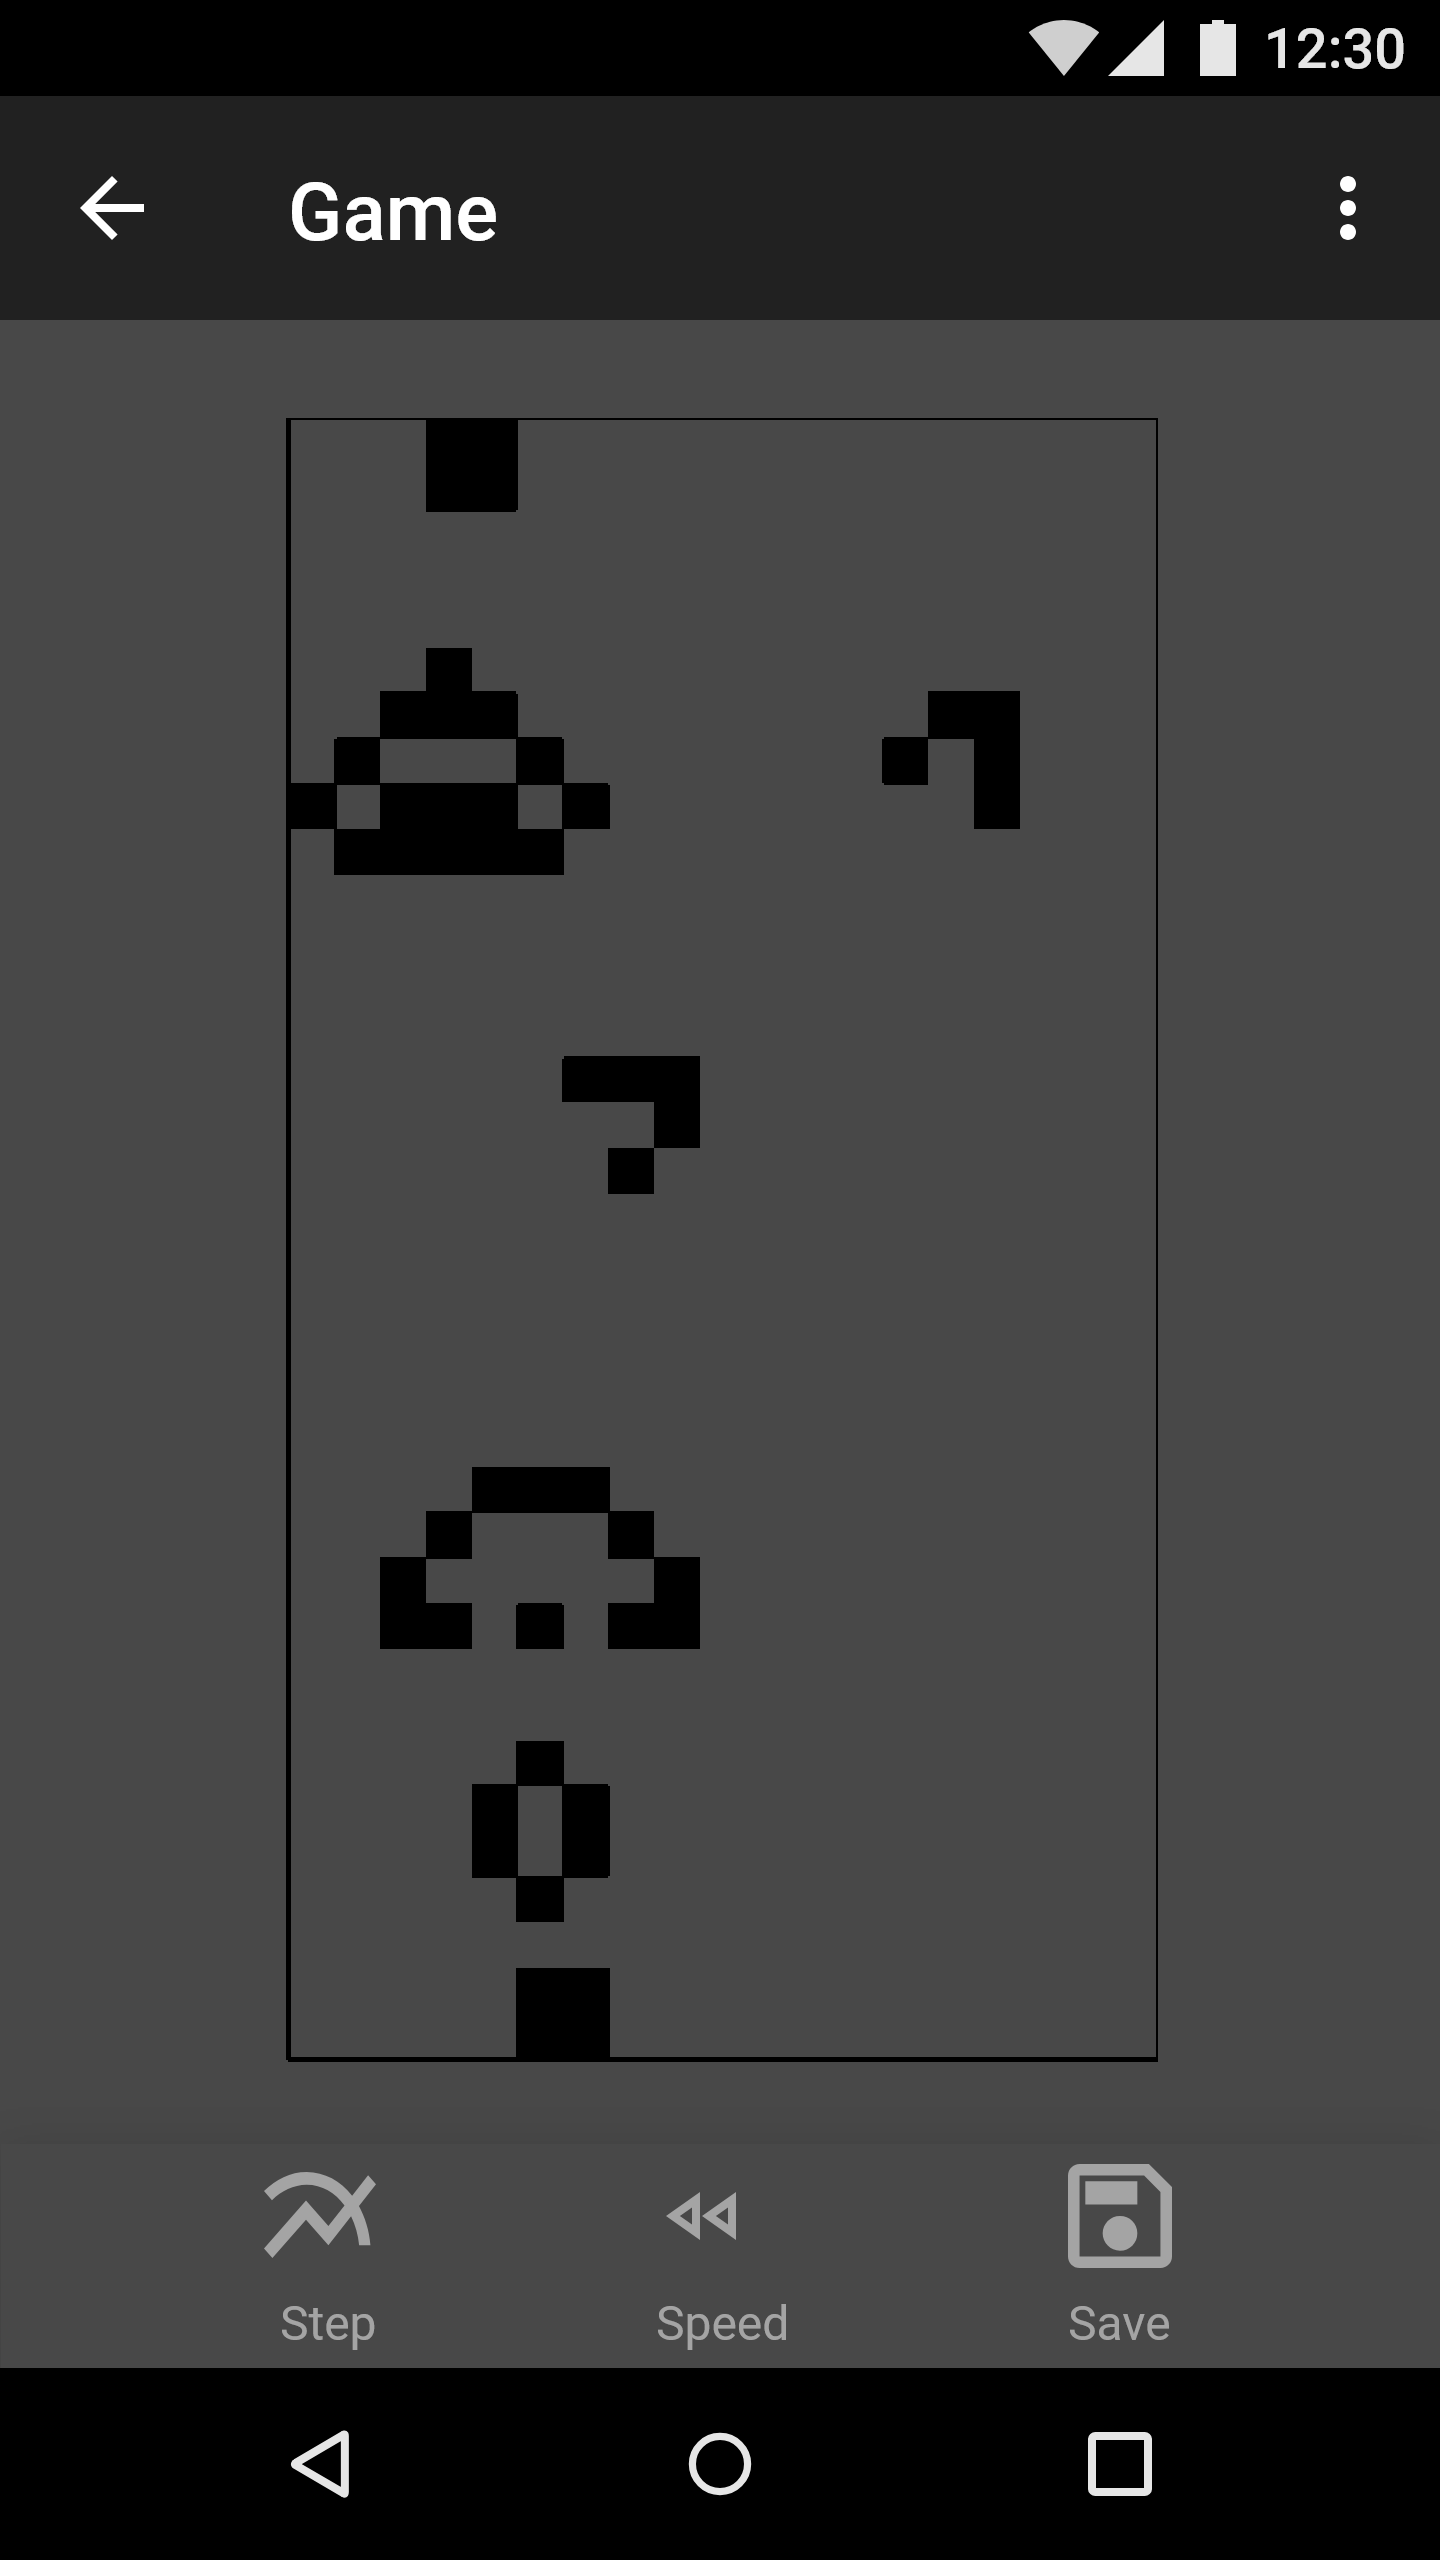
\includegraphics[width=0.33\textwidth]{Images/ui_game.png}
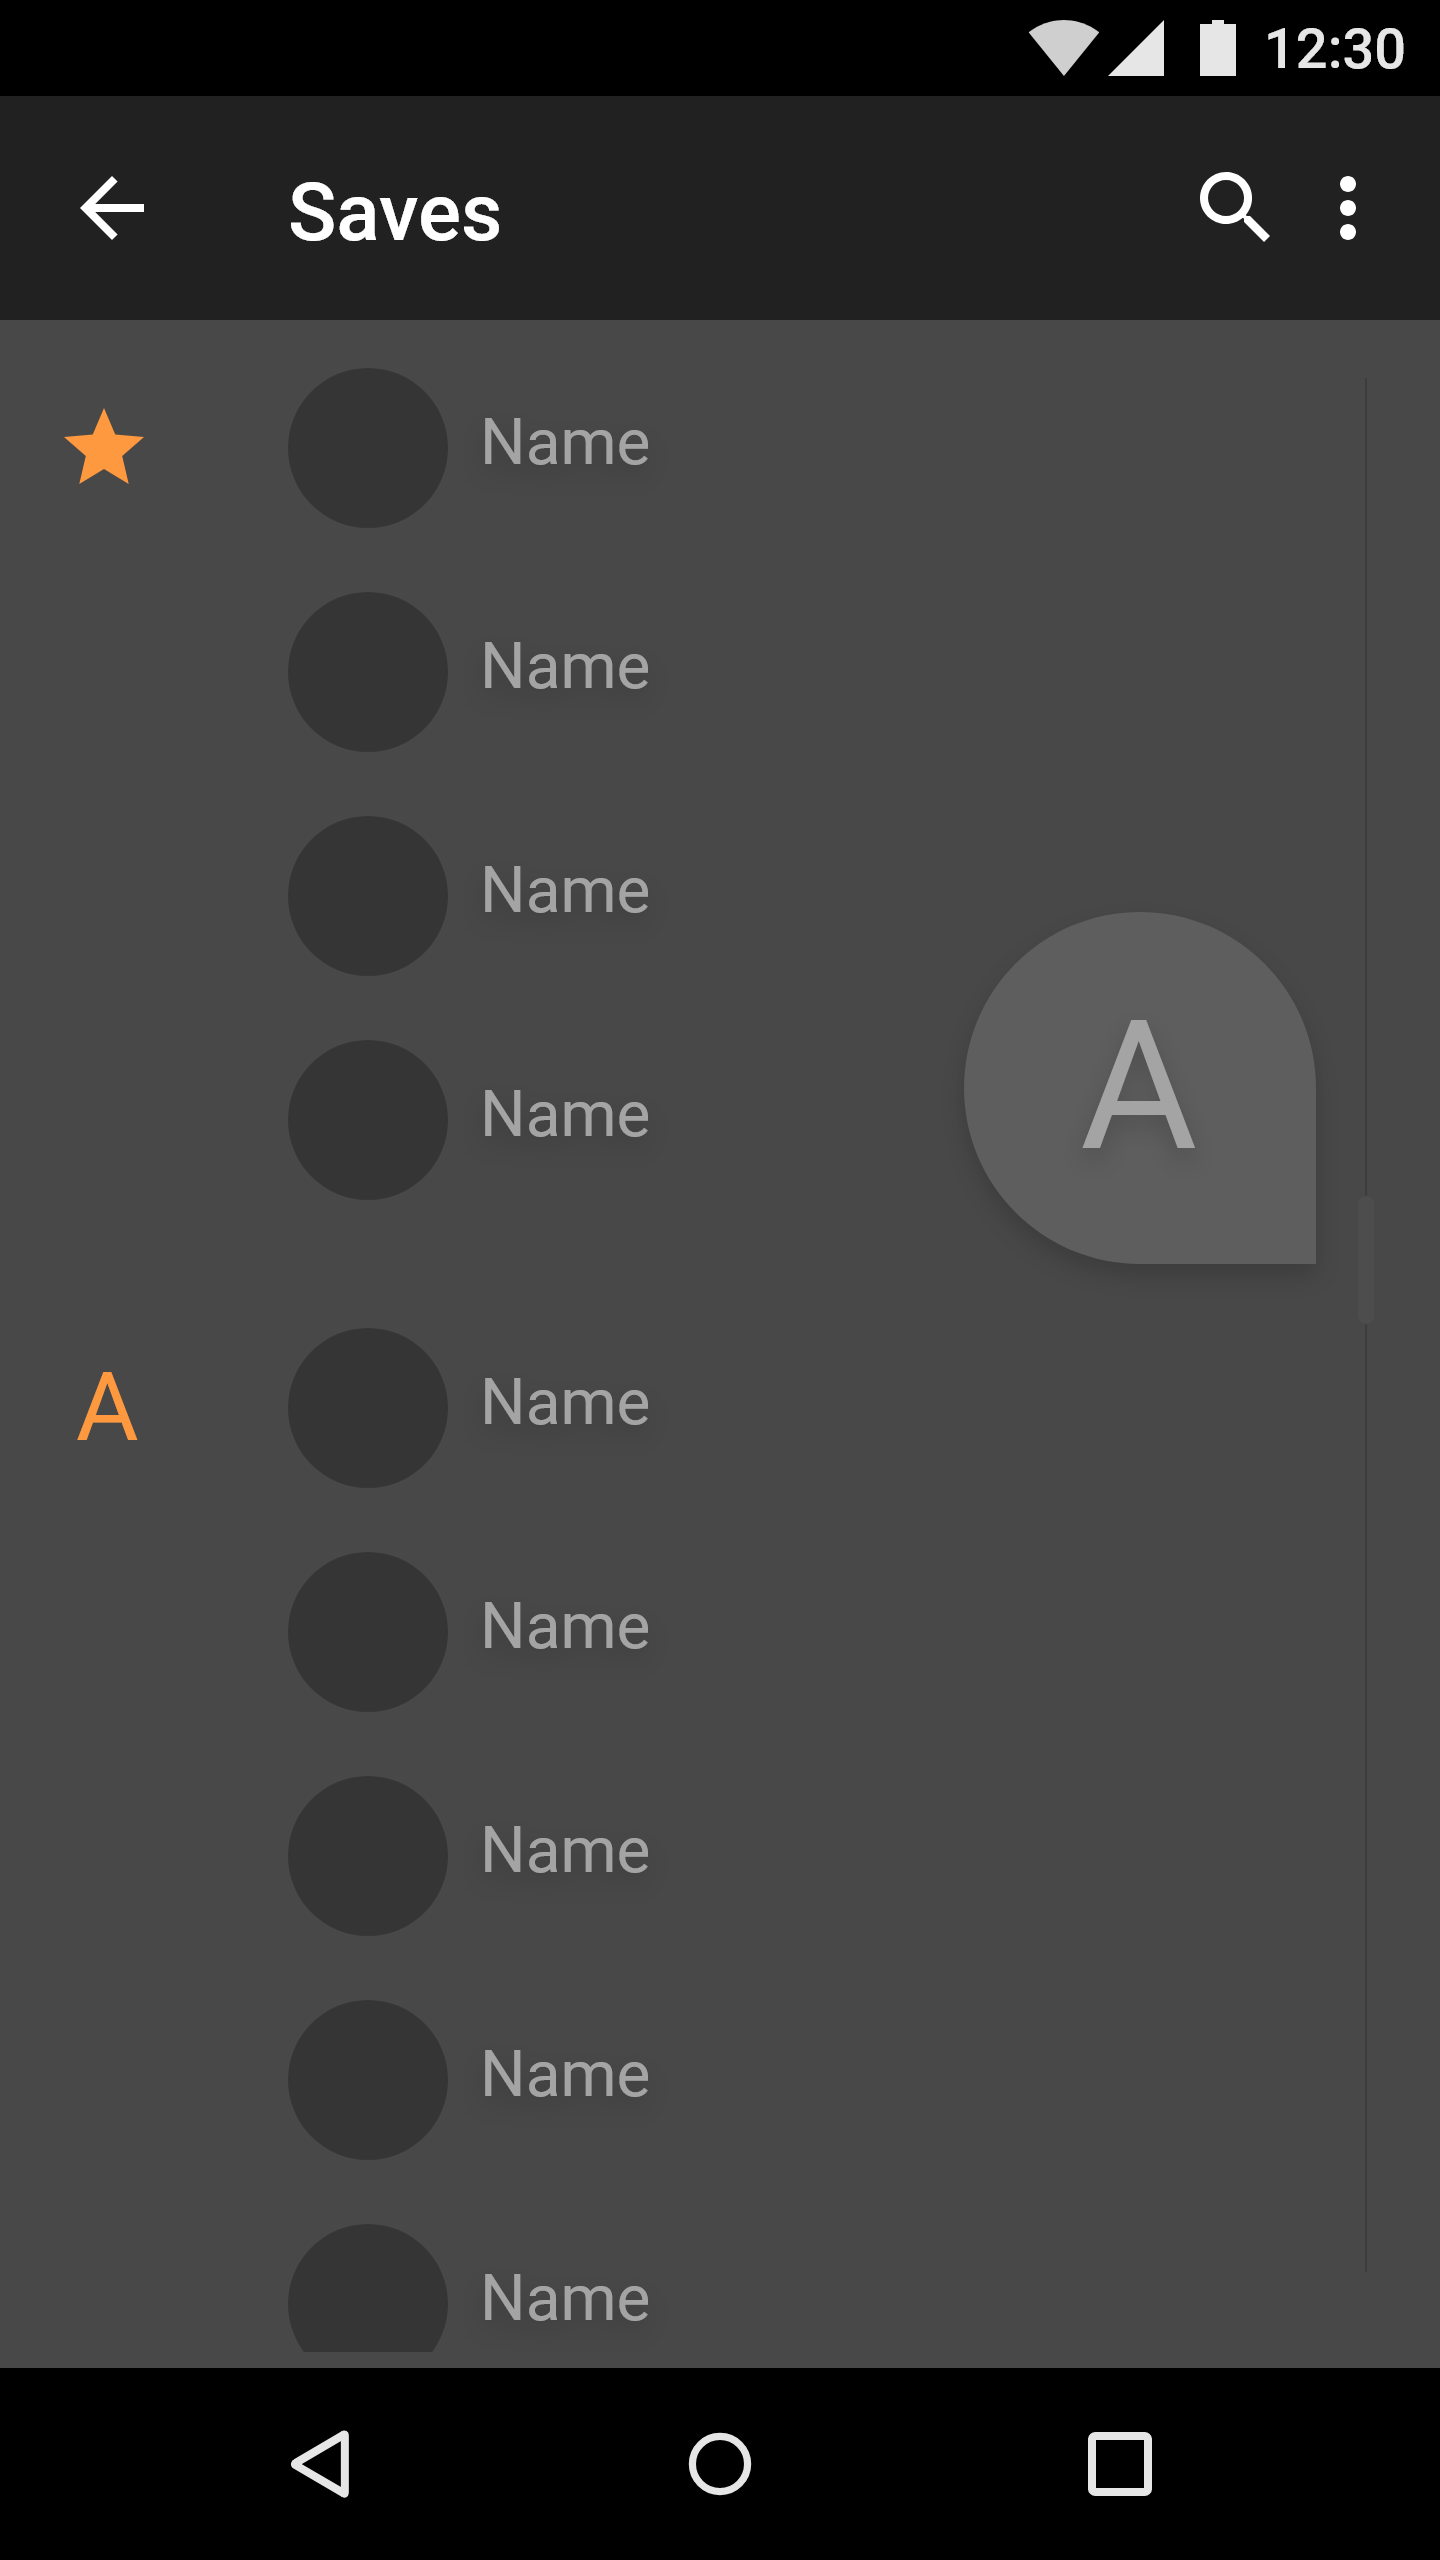
\includegraphics[width=0.33\textwidth]{Images/ui_saves.png}
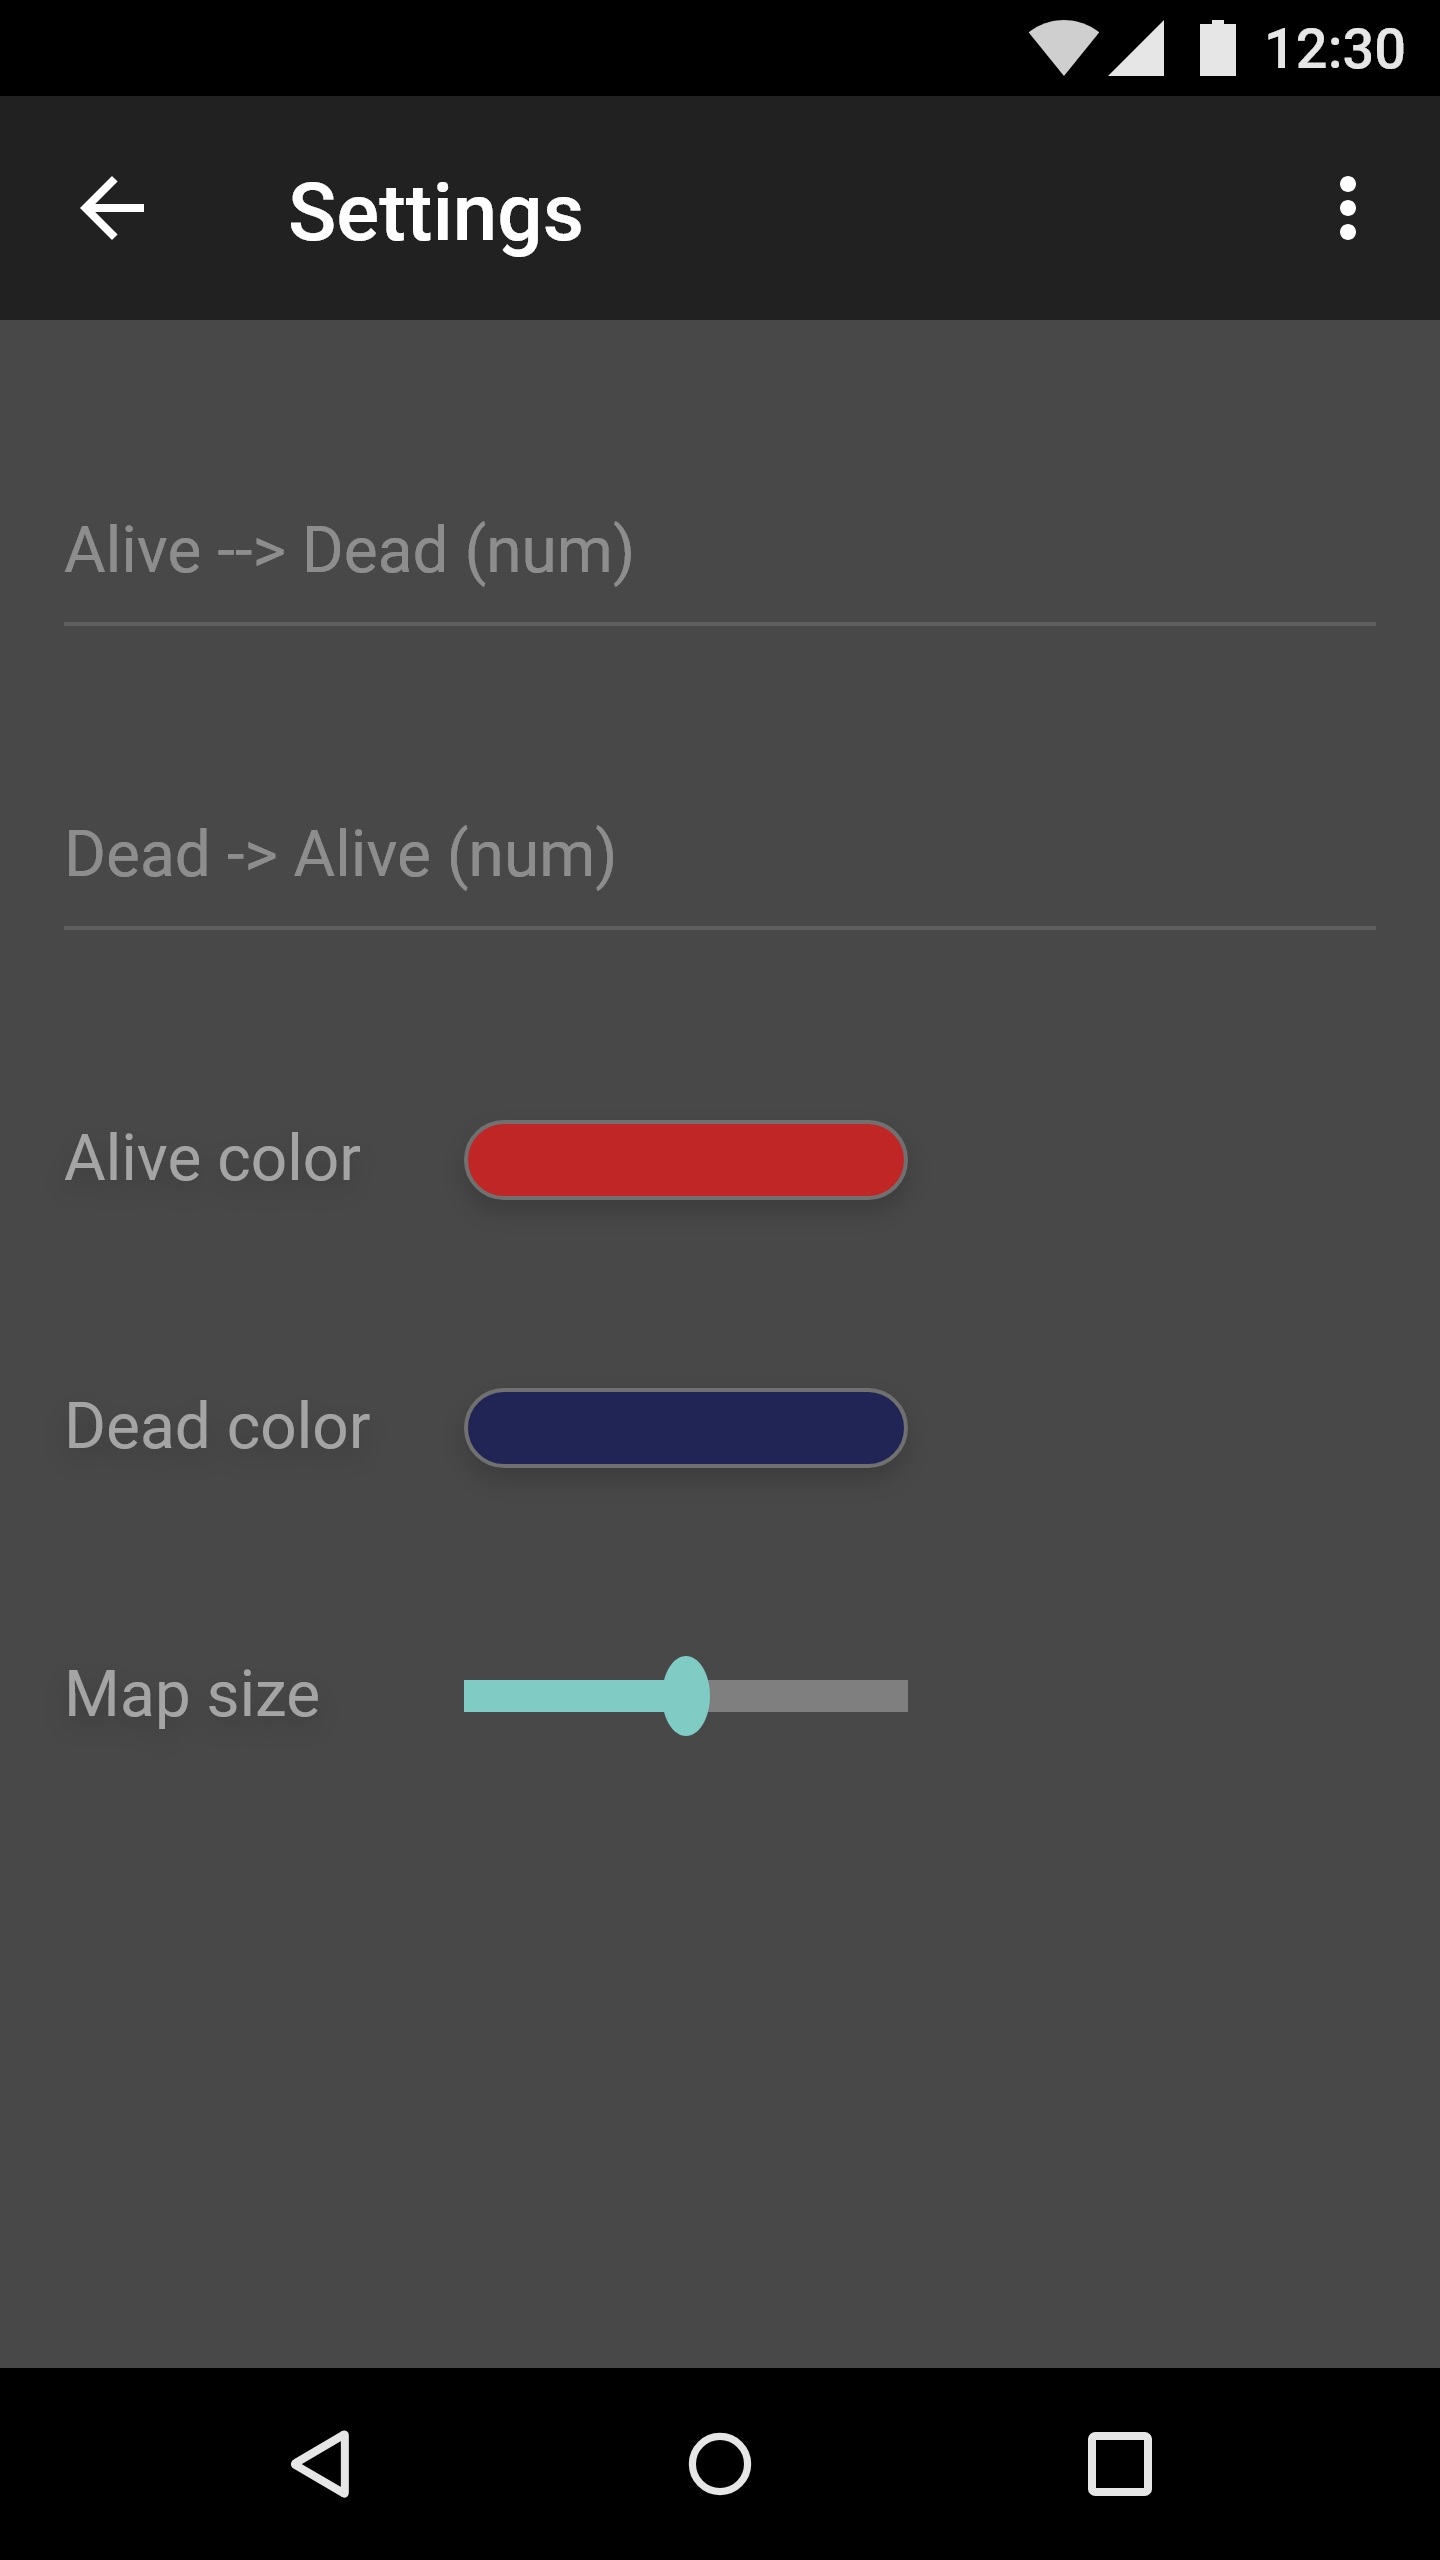
\includegraphics[width=0.33\textwidth]{Images/ui_settings.png}
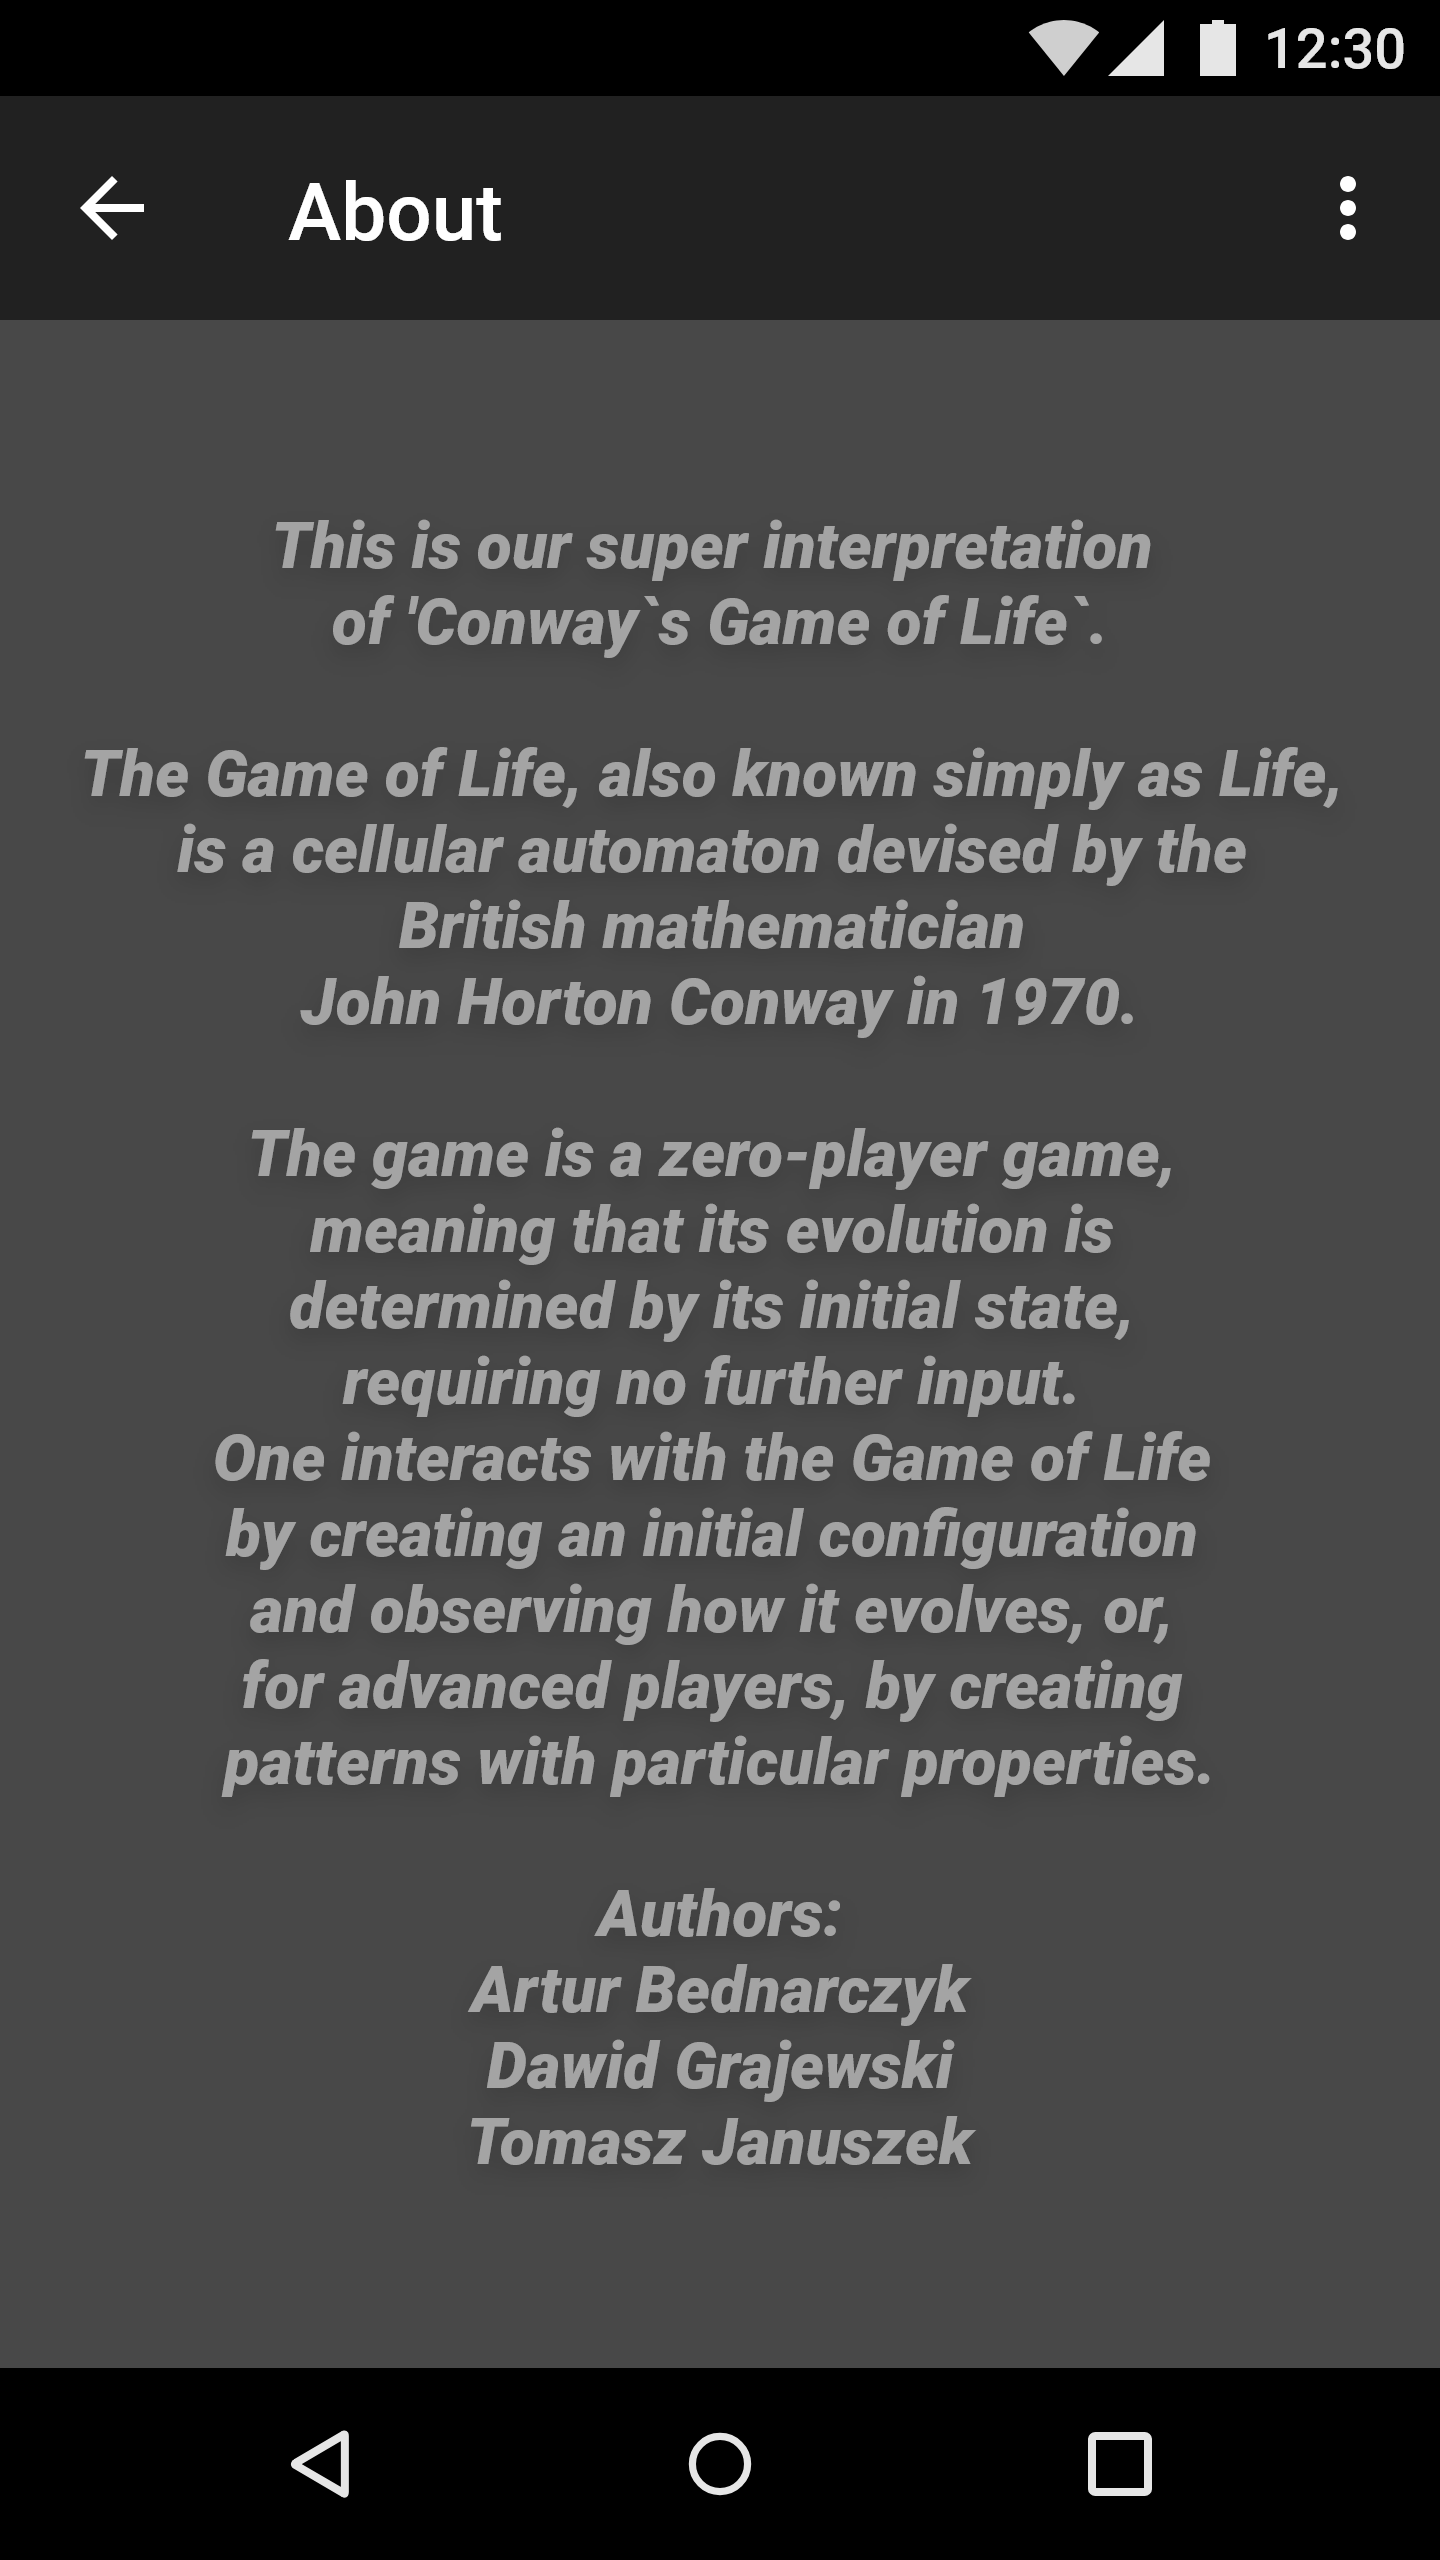
\includegraphics[width=0.33\textwidth]{Images/ui_about.png}
\section{Teoria}
\subsection{Algorytmy}
\subsubsection{Aktualizacja gry}

\section{Narzędzia}
\subsection{Kontrola wersji}
Do zarządzania kodem i wersjami projektu wykorzystujemy narzędzie Git. Korzystamy z platformy GitHub jako repozytorium dostępnego online. Dobór narzędzi służących do korzystania z repozytorium to sprawa indywidualna każdego członka zespołu, ponieważ nie ma ona wpływu na sam projekt.

\subsection{Zarzadzanie zespołem}
Trello - Kanban Board - to tutaj rozpisujemy zadania i przydzielamy je sobie, określamy również terminy i planujemy.\\


\subsection{Środowisko}
Android Studio - Kotlin \\
\section{Aplikacja}
\subsection{Architektura}

\subsection{Struktury danych}

\subsection{Schemat graficzny struktury systemu}
\subsection{Testowanie}

\end{document}